\documentclass[tikz, border=1cm]{standalone}

\usepackage{tikz}
\usetikzlibrary{calc}

\begin{document}
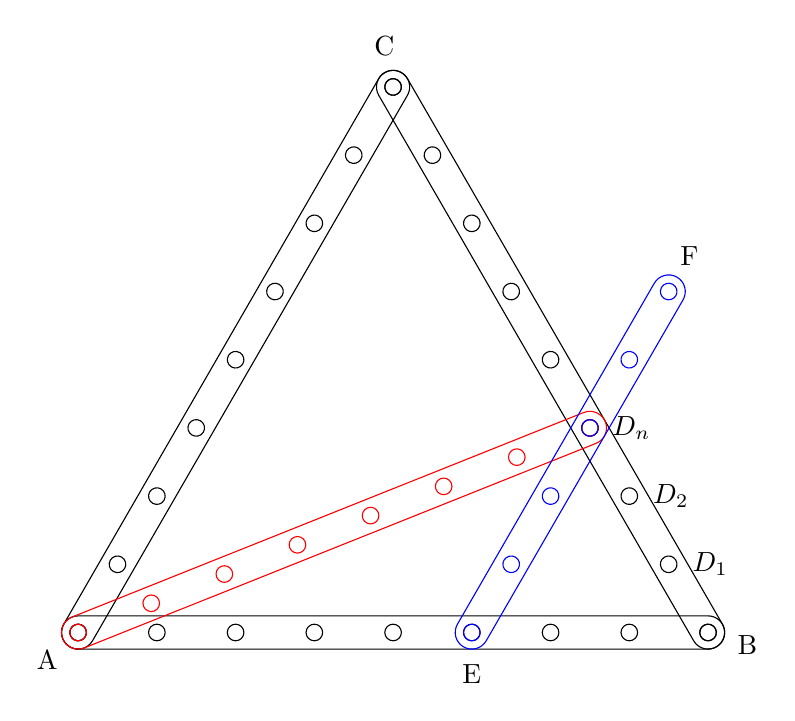
\begin{tikzpicture}

\newcommand{\rod}[4][000000] % [color][n][sep][prop]
{
 \definecolor{main}{HTML}{#1}
 \draw[main] (0,{{2*#4}})
   -- ++({#2*#3},0) arc(+90:-90:{2*#4})
   -- ++({-#2*#3},0) arc(270:90:{2*#4});
 \foreach \x in {0,1,...,#2}
  \draw[main] (\x,0) circle (#4);
}

\def\p {3pt}
\begin{scope} %AB
 \rod{8}{1}{\p}
 \path (0,0) ++(222:5*\p) node{A};
 \path (5,0) ++(270:5*\p) node{E};
\end{scope}

\begin{scope}[shift={(8,0)},rotate=120] %BC
 \rod{8}{1}{\p}
 \path (0,0) ++(222:5*\p) node{B};
 \path (1,0) ++(240:5*\p) node{$D_1$};
 \path (2,0) ++(240:5*\p) node{$D_2$};
 \path (3,0) ++(240:5*\p) node{$D_n$};
  
 \begin{scope}[shift={(8,0)},rotate=120] %CA
  \rod{8}{1}{\p}
  \path (0,0) ++(222:5*\p) node{C};
 \end{scope}
  
\end{scope}

\begin{scope}[shift={(0,0)},rotate=21.7868] %AD
 \rod[FF0000]{7}{1}{\p}
\end{scope}

\begin{scope}[shift={(5,0)},rotate=60] %EF
 \rod[0000FF]{5}{1}{\p}
 \path (5,0) ++(0:5*\p) node{F};
\end{scope}

\end{tikzpicture}
\end{document}
